% !TEX TS-program = LaTeX-shellescape
\documentclass[a4paper]{article}

\usepackage[english]{babel}
\usepackage{geometry}
\usepackage{siunitx} % voor m/s, graden Celsius
\usepackage{parskip} % geen tab na paragraafeinde
\usepackage{amsmath, amssymb} % voor equation*
\usepackage[version=4]{mhchem} % chemie
\usepackage{graphicx} % afbeeldingen
\usepackage{fancyhdr} % headers en footers
\usepackage{xcolor} % kleuren
\usepackage{pdfpages} % pdf appenden
\usepackage[bookmarksnumbered]{hyperref} % links naar tabellen en figuren
\usepackage{minted}
\usepackage[normalem]{ulem} % strikethrough
\usepackage{mdframed}
\mdfsetup{skipabove=10pt,skipbelow=10pt}
\usepackage{booktabs}

\definecolor{indigo}{rgb}{0.0, 0.25, 0.42}

\hypersetup{
  colorlinks   = true, %Colours links instead of ugly boxes
  linkcolor    = blue, %Colour of internal links
  citecolor	   = blue
}

\newcommand{\red}{\textcolor{red}}
\newcommand{\orange}{\textcolor{orange}}
\newcommand{\yellow}{\textcolor{yellow}}
\newcommand{\green}{\textcolor{green}}
\newcommand{\blue}{\textcolor{blue}}
\newcommand{\indigo}{\textcolor{indigo}}
\newcommand{\violet}{\textcolor{violet}}

\newcommand{\Ums}{[\si[per-mode=symbol]{\meter\per\second}]}
\newcommand{\Um}{[\si{\meter}]}

\newminted[ltx]{latex}{fontsize=\footnotesize, frame=single, escapeinside=||}
\newmintinline[ltxi]{latex}{}


\begin{document}
\section{Getting started with \LaTeX}
\subsection{Overleaf}
Create an account at \href{https://www.overleaf.com}{Overleaf}. Then `Create First Project' $\rightarrow$ Blank Project. Let the name of your project be `LaTeX Workshop Aardwetenschappen'. Delete all the code in the Source tab.

\subsection{A simple document}
Create a document that uses \ltxi{\documentclass{article}}. Use a4-paper. Create some sections using the commands \ltxi/\section/, \ltxi/\subsection/ and \ltxi/\paragraph/. Regularly \emph{Recompile} to see what your document looks like. 

By now your source code should look like this:
\begin{ltx}

\documentclass[a4paper]{article}

\begin{document}

\section{the first section}
some text in the first section

\section{the second section}
some text in the second section

\subsection{a subsection}
some text in the first subsection

\subsection{another}
some text in the second subsection

\paragraph{a paragraph header}
some text in a paragraph

\end{document}
\end{ltx}

\subsection{Title, date and author}
Give the document a title using the \ltxi{\title{document title}} command and an author using the \ltxi{\author{the author's name}} command. Include a date with the \ltxi{\date} command. Do not forget to add \ltxi{\maketitle} directly after \ltxi{\begin{document}}. By now the document should look like this:

\begin{ltx}

\documentclass[a4paper]{article}

\title{my article}
\author{the author}
\date{4 March 2022}

\begin{document}

\maketitle

|\vdots|

\end{document}

\end{ltx}

\subsection{Formatting text}
Recreate the text in the box, using the following commands.
\begin{itemize}
\item \ltxi{\textbf} \textbf{bold}
\item \ltxi{\textit} \textit{italic}
\item \ltxi{\underline} \underline{underline}
\item \ltxi{\sout} \sout{strikethrough} \qquad add to preamble: \ltxi{\usepackage[normalem]{ulem}}
\item \ltxi{\textsc} \textsc{Small caps}
\end{itemize}

\begin{mdframed}
We consider a \sout{horizontal} \underline{vertical cross section} of an \textsc{infinitely long polder}. The polder consists of a \textbf{confined} \textit{\textbf{aquifer}}.
\end{mdframed}

\subsection{Color}
To use color add the following code to your preamble: \ltxi{\usepackage{xcolor}}. Now you can use \ltxi{\textcolor{red}{red text here}} to make the rainbow below.

The colors used are 'red', 'orange', 'yellow', 'green', 'blue', 'indigo' and 'violet'. But 'indigo' is not one of the defined colors in LaTeX. The easiest way to use this color is to find the RGB values for indigo(dye) at \href{https://www.latexcolor.com}{latexcolor.com}. Put \ltxi{\definecolor{indigo}{rgb}{0.0, 0.25, 0.42}} in your preamble to use this new color.

\begin{center}
\huge{\red{R}\orange{a}\yellow{i}\green{n}\blue{b}\indigo{o}\violet{w}}
\end{center}

\subsection{Text size}
Use \ltxi{{\Large Text}} for larger text. Other options are:
\begin{table}[H]
\centering
\renewcommand{\arraystretch}{1.2}
\begin{tabular}{l|l}
\hline
\ltxi{\tiny} & {\tiny tiny}\\
\hline
\ltxi{\scriptsize} & {\scriptsize scriptsize}\\
\hline
\ltxi{\footnotesize} & {\footnotesize footnotesize}\\
\hline
\ltxi{\small} & {\small small}\\
\hline
\ltxi{\normalsize} & {\normalsize normalsize}\\
\hline
\ltxi{\large} & {\large large}\\
\hline
\ltxi{\Large} & {\Large Large}\\
\hline
\ltxi{\LARGE} & {\LARGE LARGE}\\
\hline
\ltxi{\huge} & {\huge huge}\\
\hline
\ltxi{\Huge} & {\Huge Huge}\\
\hline
\end{tabular}
\end{table}

Now recreate the following text:
\begin{mdframed}
We consider a {\Large Large} vertical cross section of an infinitely {\tiny tiny} polder. The polder consists of a {\Huge Huge} confined aquifer.
\end{mdframed}

\subsection{Curly braces}
Try the following commands with and without curly braces: \ltxi{\underline Test} vs \ltxi{\underline{Test}} en \ltxi{\section Titel} vs \ltxi{\section{Titel}}. What is the purpose of curly braces in \LaTeX?

\section{Math}
Recreate the following math content:
\begin{mdframed}
I can write inline math such as $a^2+b^2=c^2$. I can also give equations their own space:
\begin{equation} \label{eq:triangle}
||\vec{x} + \vec{y}|| \leq ||\vec{x}|| + ||\vec{y}||
\end{equation}
\end{mdframed}

\begin{mdframed}
\begin{equation}
\int_{a}^{b} x^2 dx = \frac{1}{3}(a^3-b^3)
\end{equation}
\end{mdframed}

\begin{mdframed}
\begin{align*}  
	q &= -\frac{k}{\mu L}\Delta p && \text{Darcy's Law} \label{eq:darcy} \\         
	\frac {\Delta p}{L} &=- \frac{150\mu}{\Phi_{\mathrm{s}}^2D_{\mathrm{p}}^2}\frac{(1-\epsilon)^2}{\epsilon ^3}u_{\mathrm{s}} && \text{Kozeny–Carman equation}
\end{align*}
\end{mdframed}

\section{Chemistry}
Use \ltxi{\usepackage[version=4]{mhchem}} for chemical formulas. Consult the documentation at \href{https://ctan.org/pkg/mhchem}{ctan.org/pkg/mhchem} (Package documentation PDF).

Now recreate the following excerpt from a geochemistry book:
\begin{mdframed}

The most fundamental of all aqueous geochemical reactions is the dissociation of water:
\ce{H2O <--> H+ + OH-}.
The pH scale for water changes with temperature. At \SI{0}{\celsius} ${\mathrm{K}_{\ce{H2O}} = 10-14.9}$ and the pH is $7.45$.

In the dissolution of fluorite the hydration role played by water is not explicitly written, but the hydration reactions and their aqueous complex can be approximated by:
\begin{align*}
\ce{Ca^2+ + 6H2O &->[H2O] Ca(H2O)6^2+\\
F^- + 6H2O &-> F(H2O)6^-}
\end{align*}
\end{mdframed}

\section{Tables}
Recreate the following tables using the \ltxi{\tabular} commmand. There exist many packages for creating tables, some of them are listed \href{https://tex.stackexchange.com/questions/12672/which-tabular-packages-do-which-tasks-and-which-packages-conflict}{here on stackexchange}.

\begin{center}
\begin{tabular}{|l|l|}
\hline
cell1 & cell2\\
\hline
cell3 & cell4\\
\hline
\end{tabular}
\end{center}

\begin{center}
\begin{tabular}{ r|c|c|c } 
 $x$ & $-2$ & $0$ & $2$  \\ 
 \hline
 $f(x)$ & $-8$ & $0$ & $8$ \\
 \hline
 $f'(x)$ & $12$ & $0$ & $12$ \\
\end{tabular}
\end{center}

\begin{table}[h!]
\centering
\begin{tabular}{|r|c|c|}
\hline
\textbf{Mineral} & Albite & Anorthite \\
\hline
\ce{SiO2} & 68.74 & 43.19\\
\hline
\ce{Na2O} & 11.82 & 0.0 \\
\hline 
\end{tabular}
\caption{Mineral compositions in oxide wt. \%}
\label{table:mineral}
\end{table}

\section{Figures}
Recreate \autoref{fig:nevadasam}. Use \ltxi{\caption} and \ltxi{width=0.5\textwidth}. The position of the figure should be at the bottom of the page if possible, otherewise approximately \emph{here} in the text or on a special page for floats.

\begin{figure}[bhp]
\centering
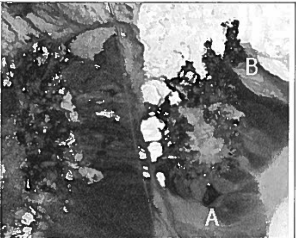
\includegraphics[width=0.5\textwidth]{kaolinite}
\caption{SAM result for Kaolinite in Cuprite, Nevada desert in the USA deribed on an AVIRIS image.}
\label{fig:nevadasam}
\end{figure}

\section{Labels and cross-referencing}
Add labels to \emph{the triangle inequality}, \emph{the table of mineral compositions} and \emph{the picture of kaolinite}. Create a list with a reference to each. \emph{hint:} use \ltxi{\usepackage[bookmarksnumbered]{hyperref}} en the command \ltxi{\autoref}.
\begin{itemize}
\item The triangle inequality: \autoref{eq:triangle}
\item Mineral compositions: \autoref{table:mineral}
\item Kaolinite: \autoref{fig:nevadasam}
\end{itemize}

\section{The bibliography}
We will now create a bibliography with a single article.

Find the article by ``\emph{Optimization of water level monitoring network in polder systems using information theory}'' on \href{https://scholar.google.com/}{scholar.google.com}, press {\LARGE ''}Cite and then BibTeX. Copy this text.

Create a new file on Overleaf called \ltxi{mybibliography.bib}. Paste the text from Google Scholar into this new file.

Now cite the article somewhere in your document, using \ltxi{\cite} and add a bibliography at the end of your document, just before \ltxi{\end{document}} \emph{hint:}
\begin{ltx}
|\vdots|
|\dots| the general solution of the well-known \emph{Polder Problem}\cite{alfonso2010}
|\vdots|
\bibliographystyle{plain}
\bibliography{literatuur.bib}
\end{document}
\end{ltx}

\begin{mdframed}
The hydraulic head distribution in the Polder satisfies the general solution of the well-known \emph{Polder Problem}\cite{alfonso2010}.
\end{mdframed}

\bibliographystyle{plain}
\bibliography{literatuur.bib}

\section{Final assignment}
Use what you have learned to recreate the following (fictional) scientific article. The solution will be made available at \href{https://www.vkuhlmann.com/latex}{vkuhlmann.com/latex}

{\Large Hints:}
\begin{enumerate}
\item The margins are 2.54cm and the document uses A4 paper.
\item Create a \ltxi{\newcommand} for \Ums{} and \Um.
\item Use \ltxi{\usepackage[version=4]{mhchem}} for chemical formulae. You can find the documentation at \href{https://ctan.org/pkg/mhchem}{ctan.org/pkg/mhchem}
\item Use the package parskip \ltxi{parskip}.
\item Use \ltxi{newpage} directly after \ltxi{tableofcontents}
\end{enumerate}

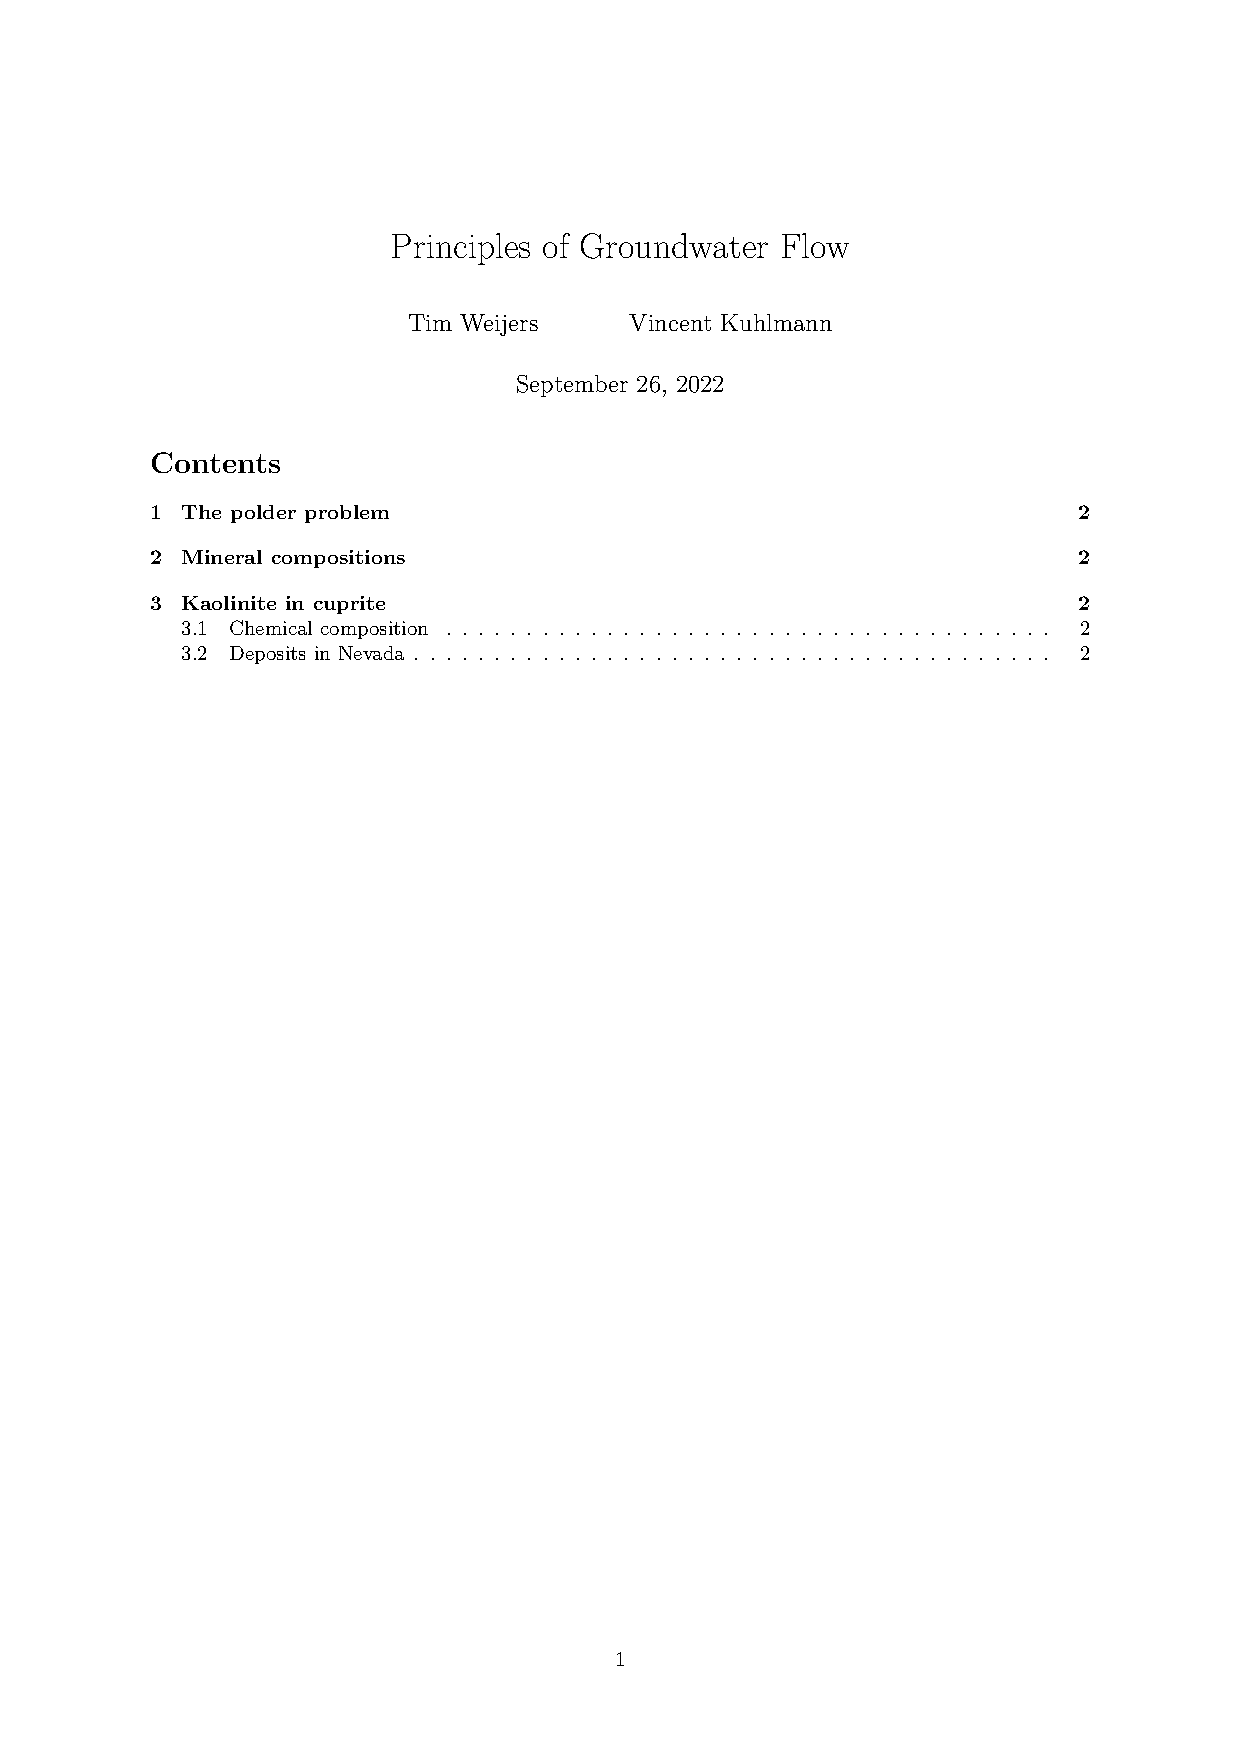
\includepdf[pages=-]{eindopdracht.pdf}





\end{document}